\documentclass[border=10pt]{standalone}
\usepackage{amsmath}
\usepackage{tikz}
\usetikzlibrary{arrows.meta, positioning, fit, backgrounds, calc}

\definecolor{wfcol}{HTML}{4FC3F7}
\definecolor{agcol}{HTML}{AB47BC}
\definecolor{toolcol}{HTML}{FFA726}
\definecolor{outputcol}{HTML}{66BB6A}

\begin{document}
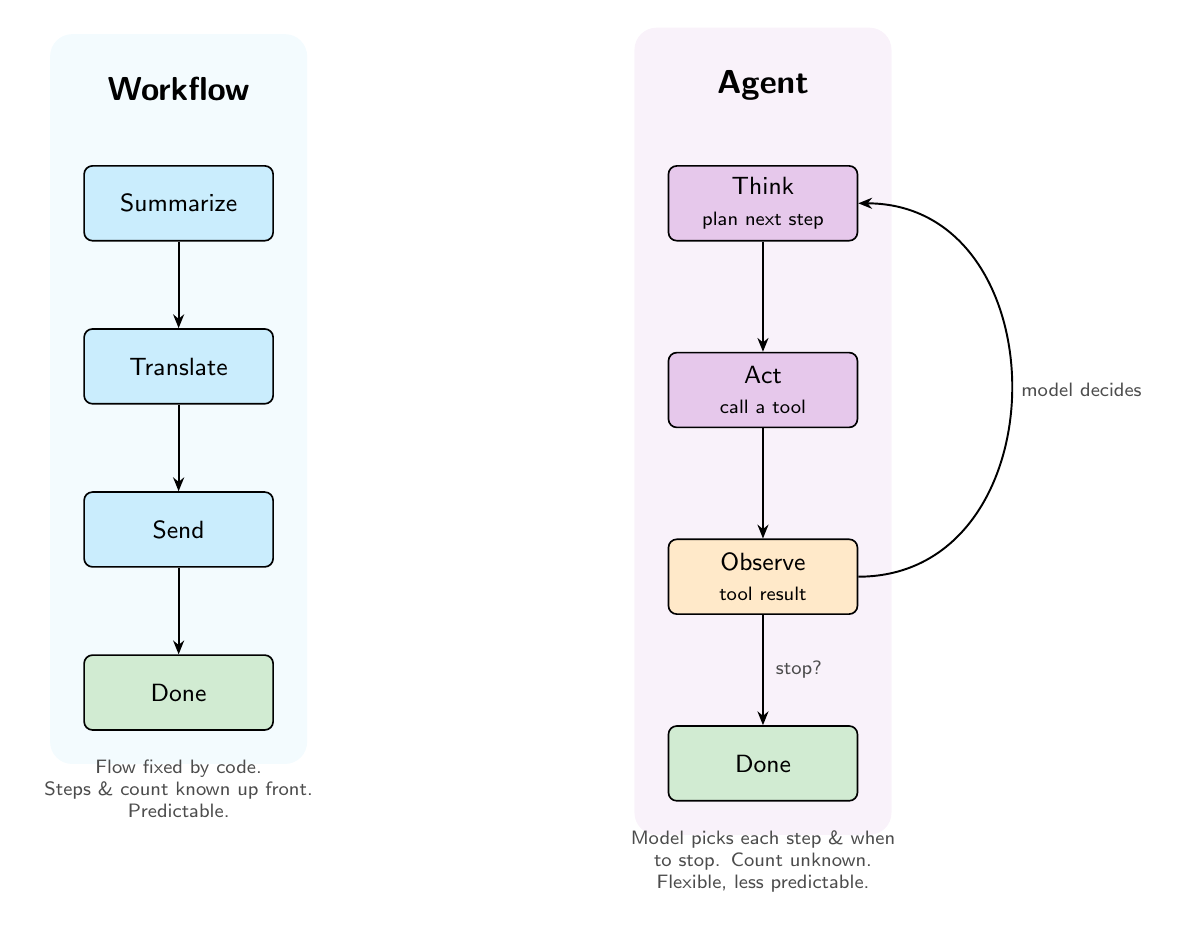
\begin{tikzpicture}[
  box/.style={draw, rounded corners=3pt, minimum width=2.4cm, minimum height=0.95cm,
    font=\sffamily\small, align=center, line width=0.6pt},
  conn/.style={-{Stealth[length=5pt, width=4pt]}, line width=0.7pt},
  annot/.style={font=\sffamily\scriptsize, text=gray!60!black},
  title/.style={font=\sffamily\bfseries\large},
]

% =================== LEFT: Workflow ===================
\node[box, fill=wfcol!30] (w1) {Summarize};
\node[box, fill=wfcol!30, below=1.1cm of w1] (w2) {Translate};
\node[box, fill=wfcol!30, below=1.1cm of w2] (w3) {Send};
\node[box, fill=outputcol!30, below=1.1cm of w3] (wend) {Done};

\draw[conn] (w1) -- (w2);
\draw[conn] (w2) -- (w3);
\draw[conn] (w3) -- (wend);

\node[title, above=0.7cm of w1] (wtitle) {Workflow};
\node[annot, below=0.25cm of wend, align=center, text width=3.6cm]
  {Flow fixed by code.\\ Steps \& count known up front.\\ Predictable.};

\begin{scope}[on background layer]
  \node[fit=(wtitle)(w1)(w2)(w3)(wend), fill=wfcol!7, rounded corners=8pt,
        inner sep=12pt] (wbox) {};
\end{scope}

% =================== RIGHT: Agent ===================
\node[box, fill=agcol!30, right=5.0cm of w1] (think) {Think\\ \scriptsize plan next step};
\node[box, fill=agcol!30, below=1.4cm of think] (act) {Act\\ \scriptsize call a tool};
\node[box, fill=toolcol!25, below=1.4cm of act] (obs) {Observe\\ \scriptsize tool result};

% loop think -> act -> observe -> think
\draw[conn] (think) -- (act);
\draw[conn] (act) -- (obs);
\draw[conn] (obs.east) to[out=0, in=0, looseness=1.4]
  node[annot, right, pos=0.5] {model decides} (think.east);

% exit when model stops
\node[box, fill=outputcol!30, below=1.4cm of obs] (agend) {Done};
\draw[conn] (obs) -- node[annot, right=1pt] {stop?} (agend);

\node[title, above=0.7cm of think] (atitle) {Agent};
\node[annot, below=0.25cm of agend, align=center, text width=3.8cm]
  {Model picks each step \& when\\ to stop. Count unknown.\\ Flexible, less predictable.};

\begin{scope}[on background layer]
  \node[fit=(atitle)(think)(act)(obs)(agend), fill=agcol!7, rounded corners=8pt,
        inner sep=12pt] (abox) {};
\end{scope}

\end{tikzpicture}
\end{document}
